% Chapter 2

\chapter{The name of chapter 2} % Main chapter title

\label{Chapter2} % for referencing this chapter elsewhere, use \ref{Chapter2}

\lhead{Chapter 2. \emph{The name of chapter 2}} % this is for the header on each page - perhaps a shortened title

%----------------------------------------------------------------------------------------

\section{A headline}

% -------------- Beginning of figure environment ----------------%
\begin{figure}[ht!]
     \centering
%
        \subfigure[foo]
        {
            \label{fig:foo}
            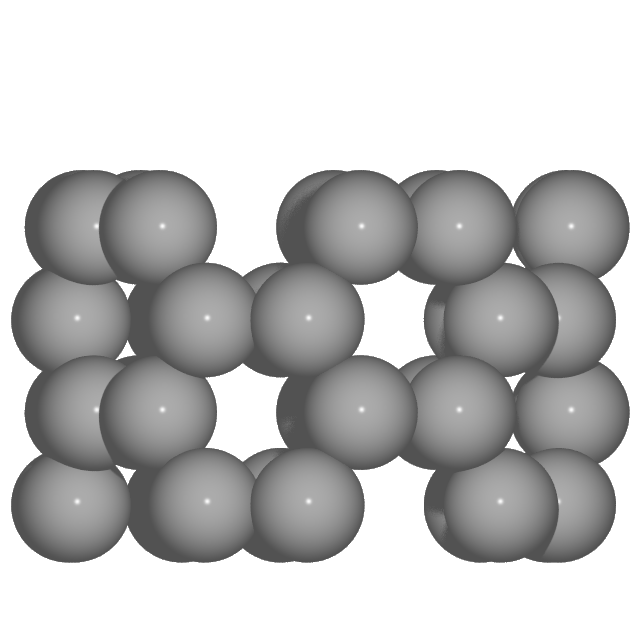
\includegraphics[width=0.3\textwidth]{./Figures/foo.png}
        }
        \hspace{0.02\textwidth}
        \subfigure[bar]
        {
            \label{fig:bar}
            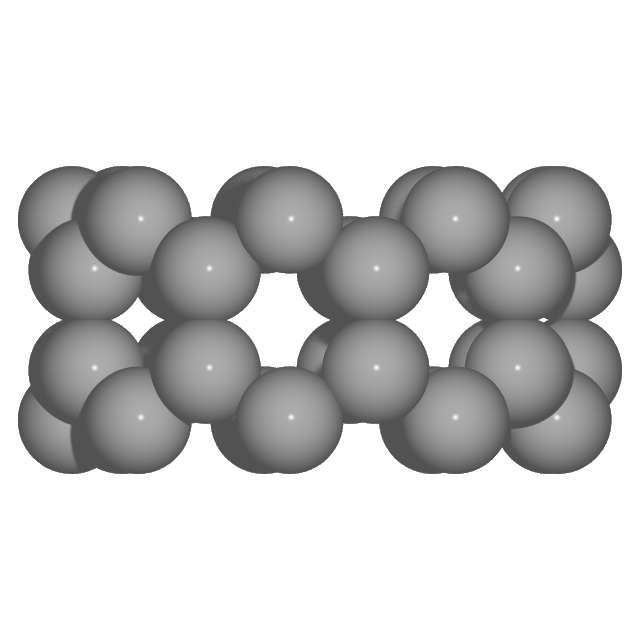
\includegraphics[width=0.3\textwidth]{./Figures/bar.png}
        }
%
    \rule{35em}{0.5pt}
    \caption[foobar]{
	Look, a foobar!
     }%
   \label{fig:foobar}
\end{figure}
% -------------- End of figure environment ----------------------%

The foo and bar is shown side by side in figure \ref{fig:foobar}...
\\
Blablalbalalkbjalkjdf.


\begin{table}
  \centering
    \begin{tabular}{ | l | c | c | c | c | c | c | c | }
      \hline
      $N_{\text{cap}}$                & 10      & 11      & 12      & 13      & 14      & 15      & 16      \\ 
      $E_{\text{cap},N_{\text{cap}}}$ [eV] & -45.505 & -45.968 & -45.981 & -46.250 & -46.181 & -46.450 & -46.303 \\ \hline \hhline{~=======}
      \multicolumn{1}{l |}{}          & 17      & 18      & 19      & 20      & 21      & 22      & 23 \\
      \multicolumn{1}{l |}{}          & -46.506 & -46.390 & -46.611 & -46.471 & -46.692 & -46.552 & -46.622  \\ \hhline{~=======}
      \multicolumn{1}{l |}{}          & 24      & 25      & 26      & 27      & 28      & 29      & 30 \\
      \multicolumn{1}{l |}{}          & -46.554 & -46.652 & -46.570 & -46.690 & -46.612 & -46.670 & -46.645 \\ \cline{2-8}
      \multicolumn{1}{l}{}
    \end{tabular}
  %\\
  \rule{35em}{0.5pt}
  \caption{
  A table, bla bla bla.
  }
  \label{tbl:coolData}
\end{table}

The cool data is shown in table \ref{tbl:coolData}...